\section{HellfireOS}
\label{sec:HellfireOS}
O HellfireOS é um sistema operacional de tempo real preemptivo que é parte constituinte
do Hellfire framework (HellfireFW). Projetado para sistemas MPSoC, possui gerenciamento
dinâmico de tarefas que conta com a proteção contra inversão de prioridades e possui as
seguintes políticas de escalonamento:
Rate Monotonic, Round Robin, Earliest Deadline First e Deadline Monotonic.\\
Dentre as bibliotecas que nos interessam consta uma LibC customizada, uma math.h com emulação
de número de ponto flutuante e parte da pilha TCP.\\
Utilizaremos o HellfireOS para controlar os sensores conectados e simulados que iremos utilizar para a nossa
prova de conceito.
\subsection{Arquitetura}
\begin{figure}[H]
	\centering
		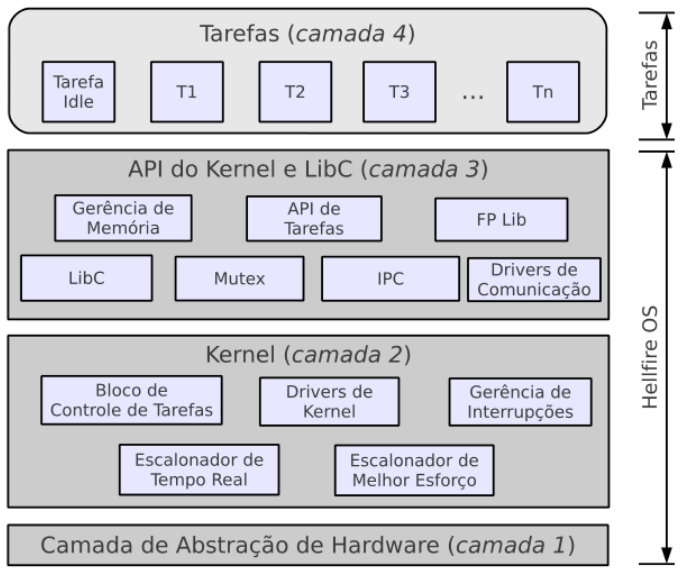
\includegraphics[width=\textwidth,height=\textheight,keepaspectratio]{fig/HellfireArch.png}
	\caption{Arquitetura em alto nível do HellfireOS.}
\end{figure}
%A API do HellfireOS é dividida em 5(cinco) grupos, a saber:
%\begin{itemize}
%	\item Manipulação de Tarefas
%	\item Exclusão Mútua
%	\item Manipulação de Memória
%	\item Comunicação entre processos
%	\item LibC
%\end{itemize}
